\documentclass{article}
\usepackage[margin=1in]{geometry}
\usepackage[linesnumbered,ruled,vlined]{algorithm2e}
\usepackage{amsfonts}
\usepackage{amsmath}
\usepackage{amssymb}
\usepackage{amsthm}
\usepackage{enumitem}
\usepackage{fancyhdr}
\usepackage{hyperref}
\usepackage{minted}
\usepackage{multicol}
\usepackage{pdfpages}
\usepackage{standalone}
\usepackage[many]{tcolorbox}
\usepackage{tikz-cd}
\usepackage{transparent}
\usepackage{xcolor}
% \tcbuselibrary{minted}

\author{Nathan Solomon}

\newcommand{\fig}[1]{
    \begin{center}
        \includegraphics[width=\textwidth]{#1}
    \end{center}
}

% Math commands
\renewcommand{\d}{\mathrm{d}}
\DeclareMathOperator{\id}{id}
\DeclareMathOperator{\im}{im}
\DeclareMathOperator{\proj}{proj}
\DeclareMathOperator{\Span}{span}
\DeclareMathOperator{\Tr}{Tr}
\DeclareMathOperator{\tr}{tr}
\DeclareMathOperator{\ad}{ad}
\DeclareMathOperator{\ord}{ord}
%%%%%%%%%%%%%%% \DeclareMathOperator{\sgn}{sgn}
\DeclareMathOperator{\Aut}{Aut}
\DeclareMathOperator{\Inn}{Inn}
\DeclareMathOperator{\Out}{Out}
\DeclareMathOperator{\stab}{stab}

\newcommand{\N}{\ensuremath{\mathbb{N}}}
\newcommand{\Z}{\ensuremath{\mathbb{Z}}}
\newcommand{\Q}{\ensuremath{\mathbb{Q}}}
\newcommand{\R}{\ensuremath{\mathbb{R}}}
\newcommand{\C}{\ensuremath{\mathbb{C}}}
\renewcommand{\H}{\ensuremath{\mathbb{H}}}
\newcommand{\F}{\ensuremath{\mathbb{F}}}

\newcommand{\E}{\ensuremath{\mathbb{E}}}
\renewcommand{\P}{\ensuremath{\mathbb{P}}}

\newcommand{\es}{\ensuremath{\varnothing}}
\newcommand{\inv}{\ensuremath{^{-1}}}
\newcommand{\eps}{\ensuremath{\varepsilon}}
\newcommand{\del}{\ensuremath{\partial}}
\renewcommand{\a}{\ensuremath{\alpha}}

\newcommand{\abs}[1]{\ensuremath{\left\lvert #1 \right\rvert}}
\newcommand{\norm}[1]{\ensuremath{\left\lVert #1\right\rVert}}
\newcommand{\mean}[1]{\ensuremath{\left\langle #1 \right\rangle}}
\newcommand{\floor}[1]{\ensuremath{\left\lfloor #1 \right\rfloor}}
\newcommand{\ceil}[1]{\ensuremath{\left\lceil #1 \right\rceil}}
\newcommand{\bra}[1]{\ensuremath{\left\langle #1 \right\rvert}}
\newcommand{\ket}[1]{\ensuremath{\left\lvert #1 \right\rangle}}
\newcommand{\braket}[2]{\ensuremath{\left.\left\langle #1\right\vert #2 \right\rangle}}

\newcommand{\catname}[1]{{\normalfont\textbf{#1}}}

\newcommand{\up}{\ensuremath{\uparrow}}
\newcommand{\down}{\ensuremath{\downarrow}}

% Custom environments
\newtheorem{thm}{Theorem}[section]

\definecolor{probBackgroundColor}{RGB}{250,240,240}
\definecolor{probAccentColor}{RGB}{140,40,0}
\newenvironment{prob}{
    \stepcounter{thm}
    \begin{tcolorbox}[
        boxrule=1pt,
        sharp corners,
        colback=probBackgroundColor,
        colframe=probAccentColor,
        borderline west={4pt}{0pt}{probAccentColor},
        breakable
    ]
    \color{probAccentColor}\textbf{Problem \thethm.} \color{black}
} {
    \end{tcolorbox}
}

\definecolor{exampleBackgroundColor}{RGB}{212,232,246}
\newenvironment{example}{
    \stepcounter{thm}
    \begin{tcolorbox}[
      boxrule=1pt,
      sharp corners,
      colback=exampleBackgroundColor,
      breakable
    ]
    \textbf{Example \thethm.}
} {
    \end{tcolorbox}
}

\definecolor{propBackgroundColor}{RGB}{255,245,220}
\definecolor{propAccentColor}{RGB}{150,100,0}
\newenvironment{prop}{
    \stepcounter{thm}
    \begin{tcolorbox}[
        boxrule=1pt,
        sharp corners,
        colback=propBackgroundColor,
        colframe=propAccentColor,
        breakable
    ]
    \color{propAccentColor}\textbf{Proposition \thethm. }\color{black}
} {
    \end{tcolorbox}
}

\definecolor{thmBackgroundColor}{RGB}{235,225,245}
\definecolor{thmAccentColor}{RGB}{50,0,100}
\renewenvironment{thm}{
    \stepcounter{thm}
    \begin{tcolorbox}[
        boxrule=1pt,
        sharp corners,
        colback=thmBackgroundColor,
        colframe=thmAccentColor,
        breakable
    ]
    \color{thmAccentColor}\textbf{Theorem \thethm. }\color{black}
} {
    \end{tcolorbox}
}

\definecolor{corBackgroundColor}{RGB}{240,250,250}
\definecolor{corAccentColor}{RGB}{50,100,100}
\newenvironment{cor}{
    \stepcounter{thm}
    \begin{tcolorbox}[
        enhanced,
        boxrule=0pt,
        frame hidden,
        sharp corners,
        colback=corBackgroundColor,
        borderline west={4pt}{0pt}{corAccentColor},
        breakable
    ]
    \color{corAccentColor}\textbf{Corollary \thethm. }\color{black}
} {
    \end{tcolorbox}
}

\definecolor{lemBackgroundColor}{RGB}{255,245,235}
\definecolor{lemAccentColor}{RGB}{250,125,0}
\newenvironment{lem}{
    \stepcounter{thm}
    \begin{tcolorbox}[
        enhanced,
        boxrule=0pt,
        frame hidden,
        sharp corners,
        colback=lemBackgroundColor,
        borderline west={4pt}{0pt}{lemAccentColor},
        breakable
    ]
    \color{lemAccentColor}\textbf{Lemma \thethm. }\color{black}
} {
    \end{tcolorbox}
}

\definecolor{proofBackgroundColor}{RGB}{255,255,255}
\definecolor{proofAccentColor}{RGB}{80,80,80}
\renewenvironment{proof}{
    \begin{tcolorbox}[
        enhanced,
        boxrule=1pt,
        sharp corners,
        colback=proofBackgroundColor,
        colframe=proofAccentColor,
        borderline west={4pt}{0pt}{proofAccentColor},
        breakable
    ]
    \color{proofAccentColor}\emph{\textbf{Proof. }}\color{black}
} {
    \qed \end{tcolorbox}
}

\definecolor{noteBackgroundColor}{RGB}{240,250,240}
\definecolor{noteAccentColor}{RGB}{30,130,30}
\newenvironment{note}{
    \begin{tcolorbox}[
        enhanced,
        boxrule=0pt,
        frame hidden,
        sharp corners,
        colback=noteBackgroundColor,
        borderline west={4pt}{0pt}{noteAccentColor},
        breakable
    ]
    \color{noteAccentColor}\textbf{Note. }\color{black}
} {
    \end{tcolorbox}
}


\fancyhf{}
\setlength{\headheight}{24pt}

\date{\today}
\title{Math 151A Homework \#2}

\begin{document}
\maketitle

\bigskip
\begin{prob}
\end{prob}
Let $p$ be some point such that $f(p)=0$. Then $g$ has a fixed point at $p$ iff $g(p)=p$.
\begin{enumerate}[label=(\alph*)]
    \item
        \begin{align*}
            f(p) = 0 &= p^4 + 2p^2 - p - 3 \\
            p + 3 - 2p^2 &= p^4 \\
            p &= \left( p + 3 - 2p^2 \right)^{1/4} \\
            p &= g_1(p)
        \end{align*}
    \item
        \begin{align*}
            f(p) = 0 &= p^4 + 2p^2 - p - 3 \\
            p + 3 - p^4 &= 2p^2 \\
            p &= \left( \frac{x+3-x^4}{2} \right)^{1/2} \\
            p &= g_2(p)
        \end{align*}
\end{enumerate}

\begin{prob}
\end{prob}
\begin{lstlisting}[language=Python]
>>> def iterate(f, p_0, n):
...     p = p_0
...     for i in range(n+1):
...             print(f"p_{i} = {p}")
...             p = f(p)
... 
>>> def g_1(x): return (3 + x - 2*x**2) ** (1/4)
... 
>>> def g_2(x): return ((3 + x - x**4) / 2) ** (1/2)
... 
>>> iterate(g_1, 1, 4)
p_0 = 1
p_1 = 1.189207115002721
p_2 = 1.0800577526675623
p_3 = 1.1496714305893827
p_4 = 1.1078205295102599
>>> iterate(g_2, 1, 4)
p_0 = 1
p_1 = 1.224744871391589
p_2 = 0.9936661590774817
p_3 = 1.228568645274987
p_4 = 0.9875064291508866
\end{lstlisting}
\bigskip
Here is a graph of $g_1$ in red and $g_2$ in blue:
\begin{center}
    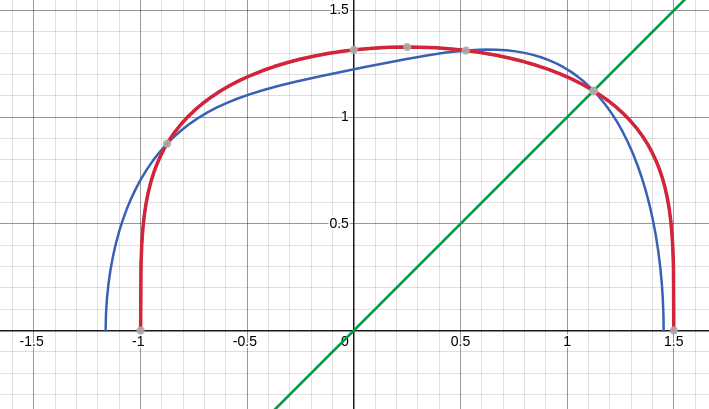
\includegraphics[width=0.5\textwidth]{Screenshot from 2024-10-18 19-52-07.png}
\end{center}
From that graph, we can see that if $p_0=1$, then FPI with either $g_1$ or $g_2$ will approximate the root $r_1 = 1.124123\dots$ (and not the root $r_2$, which is negative). After 4 iterations, FPI with $g_1$ approximates $r_1$ to be $1.107821$ and FPI with $g_2$ approximates that same root as $0.987506$. Therefore, I think $g_1$ is better for approximating the root $r_1$.

\bigskip
\begin{prob}
\end{prob}
There are 4 hypotheses needed to show existence and uniqueness of fixed points. If the following are all true:
\begin{itemize}
    \item $g \in C([a,b])$
    \item $g(x) \in [a,b]$ for all $x \in [a,b]$
    \item $g'(x)$ exists when $x \in (a,b)$
    \item there exists $k \in (0, 1)$ such that $\abs{g'(x)} \leq k$ for all $x \in (a,b)$
\end{itemize}
then $g$ has a unique fixed point on $[a,b]$. If the first two criteria are true, then $g$ has a fixed point on $[a,b]$, but that alone would not guarantee it is unique.
\par
Let $a = 0, b = 2 \pi, g(x) = \pi + 0.5 \sin (x/2)$. Then $g$ is continuous on $[a,b]$. Since the sine of a real number is always in $[-1, 1]$, the image $g([a,b])$ is in $[\pi -0.5, \pi + 0.5]$. $g$ is differentiably everywhere, and $g'(x) = 0.25 \cos(x/2)$. So if $k = 0.25$, then $\abs{g'(x)}$ is always less than or equal to $k$.
\par
All 4 hypotheses are satisfied, so $g$ has a unique fixed point on $[0, 2\pi]$.

\bigskip
\begin{prob}
\end{prob}
\begin{lstlisting}[language=Python]
>>> from math import sin, cos
>>> def f(x): return -x**3 - cos(x)
... 
>>> def f_prime(x): return -3 * x**2 + sin(x)
... 
>>> p = -1
>>> iteration = 0
>>> tolerance = 1e-10
>>> max_iterations = 40
>>> while abs(f(p)) > tolerance and iteration < max_iterations:
...     iteration += 1
...     p -= f(p) / f_prime(p)
...     print(f"{iteration=}\t {p=}\t residual={abs(f(p))}")
... 
iteration=1	 p=-0.880332899571582	 residual=0.04535115463649053
iteration=2	 p=-0.8656841631760818	 residual=0.0006323133963189731
iteration=3	 p=-0.865474075952977	 residual=1.289199819121123e-07
iteration=4	 p=-0.8654740331016162	 residual=5.218048215738236e-15
\end{lstlisting}
\bigskip
Newton's method converges very quickly. The approximation after two iterations is $p_2 = -0.8656841631760818$ and the residual is $f(p_2) = 0.0006323133963189731$. Newton's method only works because we chose a good value for $p_0$ though. If $p_0$ were zero, then $f(p_0)$ would be nonzero and $f'(p_0)$ would be zero, so $p_1 = p_0 - \frac{f(p_0)}{f'(p_0)}$ would be undefined.

\bigskip
\begin{prob}
\end{prob}
\begin{lstlisting}[language=Python]
>>> from math import cos
>>> def f(x): return -x**3 - cos(x)
... 
>>> p = [-1, 0]
>>> while len(p) <= 3:
...     p.append((p[-2] * f(p[-1]) - p[-1] * f(p[-2])) / (f(p[-1]) - f(p[-2])))
... 
>>> for i in range(len(p)):
...     print(f"p_{i} = {p[i]} residual={abs(f(p[i]))}")
... 
p_0 = -1 residual=0.45969769413186023
p_1 = 0 residual=1.0
p_2 = -0.6850733573260451 residual=0.45285023447500383
p_3 = -1.252076488909229 residual=1.649523592018598
\end{lstlisting}
After 2 iterations, our approximation ($p_3$) is pretty bad, but if we kept going, it would eventually converge:
\begin{lstlisting}[language=Python]
p_4 = -0.8072055385060928	residual=0.16556011526065983
p_5 = -0.8477837694325692	residual=0.05231270017050571
p_6 = -0.8665281869207425	residual=0.0031747088825289094
p_7 = -0.8654557261640932	residual=5.5076148661736823e-05
p_8 = -0.8654740143806453	residual=5.632275656974883e-08
p_9 = -0.8654740331019471	residual=1.0009770790020411e-12
p_10 = -0.8654740331016145	residual=2.220446049250313e-16
\end{lstlisting}

\bigskip
\begin{prob}
\end{prob}
Assume $f'(p_0) \neq 0$, and define $g(x) = x - f(x) / f'(p_0)$. Let $p_1 = g(p_0), p_2 = g(p_1)$, and so on. $f$ is continuous on $[a,b]$ and $f'(p_0)$ is assumed to be nonzero, so $g$ is also continuous on $[a,b]$
\par
Suppose $p_n$ converges to $p$ as $n$ goes to infinity. By Taylor's theorem,
\[ g(x) = g(x_0) + g'(\xi_x) \cdot (x - x_0) \]
for some $\xi_x$ between $x_0$ and $x$. If we let $x = p_{n-1}$ and $x_0 = p_0$, that equation becomes
\[ g(p_{n-1}) = g(p) + g'(\xi_n) \cdot (p_{n-1} - p) \]
(for some $\xi_n$ between $p_{n-1}$ and $p$). That simplifies to
\[ p_n = p + g'(\xi_n) \cdot (p_{n-1} - p), \]
which can be rewritten as
\[ g'(\xi_n) = \frac{p_n - p}{(p_{n-1} - p)}. \]
Since $\xi_n$ is between $p_{n-1}$ and $p$, and $p_n$ converges to $p$, $\xi_n$ must also converge to $p$. The function $g'$ is continuous (because $g'(x) = 1 - f'(x) / f'(p_0)$, and $f$ is coninuously differentiable), so that means $g'(\xi_n)$ converges to $g'(p) = 1 - f'(p) / f'(p_0)$. We are given that $f'(p) \neq f'(p_0)$, so
\[ \lim_{n \rightarrow \infty} \frac{\abs{p_n-p}}{\abs{p_{n-1}-p}} = \abs{g'(p)} > 0. \]
We do not have enough information to show that $L < 1$, where $L := \abs{g'(p)}$, but if we assume $L < 1$, then we have shown $p_n$ converges linearly to $p$.
\bigskip
\begin{prob}
\end{prob}
Note thar for this question, there is some ambiguity about whether to start with $p_0$ or $p_1$ for Newton's method. I chose to ignore the given $p_1=5$ for Newton's method, and instead start with $p_0$.
\par
Here is the python program and output I used for this problem. I took out the line that attempted to use the variation of Newton's method from problem 6 with $p_0=-5$ to find the root, because that did not converge.

\bigskip
\begin{lstlisting}[language=Python]
#!/usr/bin/env python3
from math import cos, sin

def f(x): return x + cos(x)

def f_prime(x): return 1 - sin(x)

def newtons_method(f, f_prime, p_0, tolerance, weird_version=False):
    if weird_version:
        print(f"\nVariation of Newton's method from problem 6")
    else:
        print(f"\nNewton's method")
    print(f"{p_0=}\t{tolerance=}\n{'='*53}")
    i = 0
    p = p_0
    while abs(f(p)) > tolerance:
        i += 1
        if weird_version:
            p -= f(p) / f_prime(p_0)
        else:
            p -= f(p) / f_prime(p)
        print(f"p_{i:02} = {p:>16.10f},  residual = {abs(f(p)):>16.10f}")

def secant_method(f, p_0, p_1, tolerance):
    print(f"\nSecant method")
    print(f"{p_0=}\t{p_1=}\t{tolerance=}\n{'='*53}")
    p = [p_0, p_1]
    while abs(f(p[-1])) > tolerance:
        p.append((p[-2]*f(p[-1])-p[-1]*f(p[-2])) / (f(p[-1])-f(p[-2])))
    for i in range(len(p)):
        print(f"p_{i:02} = {p[i]:>16.10f},  residual = {abs(f(p[i])):>16.10f}")

newtons_method(f, f_prime, -5, 1e-10)
secant_method(f, -5, 5, 1e-10)
newtons_method(f, f_prime, -.9, 1e-10)
newtons_method(f, f_prime, -.9, 1e-10, weird_version=True)
secant_method(f, -.9, 5, 1e-10)
\end{lstlisting}
\bigskip
\begin{lstlisting}[language=Python]
Newton's method
p_0=-5	tolerance=1e-10
=====================================================
p_01 =   109.8205607048,  residual =   108.8296839085
p_02 =   -15.9607775611,  residual =    16.9289898794
p_03 =     6.6151154617,  residual =     7.5605305903
p_04 =    -4.6000997047,  residual =     4.7121531554
p_05 =   743.6197251930,  residual =   743.0281085215
p_06 = -3090.7583906372,  residual =  3089.9158322043
p_07 =  3606.1400727092,  residual =  3607.0578723786
p_08 =  1024.2182226354,  residual =  1025.2164816044
p_09 =   -65.2592470776,  residual =    66.0148654568
p_10 =   -25.3714027324,  residual =    24.3997474637
p_11 =    -5.6369297160,  residual =     4.8385854382
p_12 =     6.5264723344,  residual =     7.4970237282
p_13 =    -3.3496519727,  residual =     4.3280855996
p_14 =     2.1051947425,  residual =     1.5958713194
p_15 =    -9.3409121107,  residual =    10.3373974311
p_16 =     0.1974775656,  residual =     1.1780421553
p_17 =    -1.2681072761,  residual =     0.9700191926
p_18 =    -0.7718165872,  residual =     0.0551716918
p_19 =    -0.7393136716,  residual =     0.0003825038
p_20 =    -0.7390851447,  residual =     0.0000000193
p_21 =    -0.7390851332,  residual =     0.0000000000

Secant method
p_0=-5	p_1=5	tolerance=1e-10
=====================================================
p_00 =    -5.0000000000,  residual =     4.7163378145
p_01 =     5.0000000000,  residual =     5.2836621855
p_02 =    -0.2836621855,  residual =     0.6763747448
p_03 =    -1.0593324054,  residual =     0.5698780527
p_04 =    -0.7046391719,  residual =     0.0572061591
p_05 =    -0.7369962894,  residual =     0.0034943006
p_06 =    -0.7391013273,  residual =     0.0000271027
p_07 =    -0.7390851257,  residual =     0.0000000125
p_08 =    -0.7390851332,  residual =     0.0000000000

Newton's method
p_0=-0.9	tolerance=1e-10
=====================================================
p_01 =    -0.7438928778,  residual =     0.0080548285
p_02 =    -0.7390902113,  residual =     0.0000084988
p_03 =    -0.7390851332,  residual =     0.0000000000

Variation of Newton's method from problem 6
p_0=-0.9	tolerance=1e-10
=====================================================
p_01 =    -0.7438928778,  residual =     0.0080548285
p_02 =    -0.7393761353,  residual =     0.0004870559
p_03 =    -0.7391030189,  residual =     0.0000299338
p_04 =    -0.7390862335,  residual =     0.0000018415
p_05 =    -0.7390852009,  residual =     0.0000001133
p_06 =    -0.7390851374,  residual =     0.0000000070
p_07 =    -0.7390851335,  residual =     0.0000000004
p_08 =    -0.7390851332,  residual =     0.0000000000

Secant method
p_0=-0.9	p_1=5	tolerance=1e-10
=====================================================
p_00 =    -0.9000000000,  residual =     0.2783900317
p_01 =     5.0000000000,  residual =     5.2836621855
p_02 =    -0.6046951156,  residual =     0.2179803505
p_03 =    -0.8458696397,  residual =     0.1827890735
p_04 =    -0.7358710590,  residual =     0.0053752920
p_05 =    -0.7390133888,  residual =     0.0001200704
p_06 =    -0.7390851842,  residual =     0.0000000854
p_07 =    -0.7390851332,  residual =     0.0000000000
\end{lstlisting}
\begin{enumerate}[label=(\alph*)]
    \item With $p_0 = -5$, Newton's method took 21 iterations to reach the desired tolerance. With $p_0=-5$ and $p_1=5$, the secant method took only 7 iterations. With $p_0 = -5$, the variation of Newton's method from problem 6 diverged, which I believe is related to the fact that we couldn't prove $L < 1$ in problem 6. When $L > 1$, the method will ``diverge linearly" instead of converging linearly.
        \par
        With $p_0 = -0.9$, Newton's method took 3 iterations to reach the desired tolerance. With $p_0=-0.9$ and $p_1=5$, the secant method took 6 iterations. With $p_0 = -0.9$, the variation of Newton's method (from problem 6) took 7 iterations.
    \item When $p_0$ was $-5$ and $p_1$ was $5$, the approximations given by Newton's method and the secant method were -0.739085133215161 (residual 0.000000000000000) and -0.739085133215134 (residual 0.000000000000045), respectively.
        \par
        To obtain these results, I modified the code above to print with more precision -- otherwise the approximations from each method would be the same.
    \item See the program output above.
\end{enumerate}
Newton's method converges quadratically, which makes it very good, but only if $p_0$ is chosen well. When $p_0$ was 5, it took a while to get close to the answer, but once it did get close, it converged super fast. The variation of Newton's method didn't converge at all, because $f'(p_0)$ was almost exactly zero. On the other hand, when we chose $p_0 = -0.9$, Newton's method converged super fast (only 3 iterations), and the variation of Newton's method converged linearly. The secant method, on the other hand, converged in 7 iterations when $p_0$ was $-5$, and in 6 iterations when $p_0$ was $-0.9$. The secant method is more consistent because it doesn't depend as much on the initial guess, but it doesn't have the advantage of converging quadratically.

\end{document}
